%!TEX root = ../paper.tex

\section{Evaluation}
\label{sec:evaluation}

The following sections show the evaluation of our approach.
We start with defining our evaluation measures and then evaluate our two classifiers and relevant design decisions.

\subsection{Evaluation Measures}
\label{sub:evaluation_measures}
We use the following measures to evaluate our approach:
As already mentioned in a previous section, the demand classifier can be optimized for either precision or recall, depending on the use case.
Therefore, we consider three values:

\begin{align*}
	\emph{Precision of the demand classifier}~P_{demand} 			&= \frac{correct~predicted~demands}{predicted~demands} \\
	\emph{Recall of the demand classifier}~R_{demand} 				&= \frac{correct~predicted~demands}{all~demand~posts} \\
	\emph{Overall precision for both classes}~P_{all} &= \frac{correct~predictions}{all~predictions} \\
\end{align*}

This measures capture the most important aspects of our system: If we predict a demand, how likely is it really a demand post ($P_{demand}$), and how many of all demand posts can we actually find ($R_{demand}$).
Finally, the overall precision ($P_{all}$) of the demand classifier is usually quite high because of the data skew in the demand tagging.

For example, a tagger, which always returns ``no-demand'' has a relatively high overall precision of $\frac{406}{445}$ = $91.24~\%$, as seen in Table~\ref{table:data_overview}.
However, we left this in for the sake of completeness and take all three measure in count to evaluate demand classifier performance.
Since there is no such data skew in the product classifier, the overall precision is sufficient to describe the product classifier performance.

\subsection{Results}
\label{sub:results}

\subsubsection{Demand Classifier}
\label{ssub:demand_classifier}

We optimized our demand classifier with respect to the demand precision.
Table~\ref{table:demand_evaluation} shows that we classify 88~\% of the posts, which express a demand, correctly.
We measured this number by doing a cross validation on the tagged posts.
Cross validations means, that we split the data set in ten parts, then run the feature extraction and the learning phase on $9 / 10$ of the data to predict one the remaining $1 / 10$.
This is done repeatedly for all ten parts.
By optimizing for precision we make sure to decrease the work load of the salesmen: If we propose a post, we are quite sure, that the users needs something.

\begin{table}[h]
	\centering
	\begin{tabular}{lc}
		\hline
		\textbf{Metric} & \textbf{Result}  \\
		\hline
		\hline
		$P_{demand}$ & 88~\% \\
		\hline
		$R_{demand}$ & 51~\%  \\
		\hline
		$P_{all}$ & 93~\%  \\
		\hline
	\end{tabular}
	\caption{Cross validation results on demand classifier}
	\label{table:demand_evaluation}
\end{table}

\subsubsection{Product Classifier}
\label{ssub:product_classifier}

As we said before, linear classifiers performed best for the product classification.
Because they differ only marginally, we evaluate using three linear classifiers: Logistic Regression, Perceptron, and Support Vector Machines.
We compare these classifiers with a baseline approach (k-nearest-neighbor classification), see Figure~\ref{fig:product_eval}.
In this figure you can see the four classifiers, which are predicting exactly one of the four products for each post.
We evaluate two different cases:
First, we evaluate only on posts that we tagged as belonging to one of the four products.
Second, we evaluate on all posts, so that the classifier sometimes has to predict ``NONE''.
Of course this value is lower than the first one, because the classifier can now also wrongly predict the ``NONE'' class.
This case is nearer to the real world scenario, since not every LinkedIn post we have crawled can be mapped to one of the product classes.

\begin{figure}
	\begin{center}
		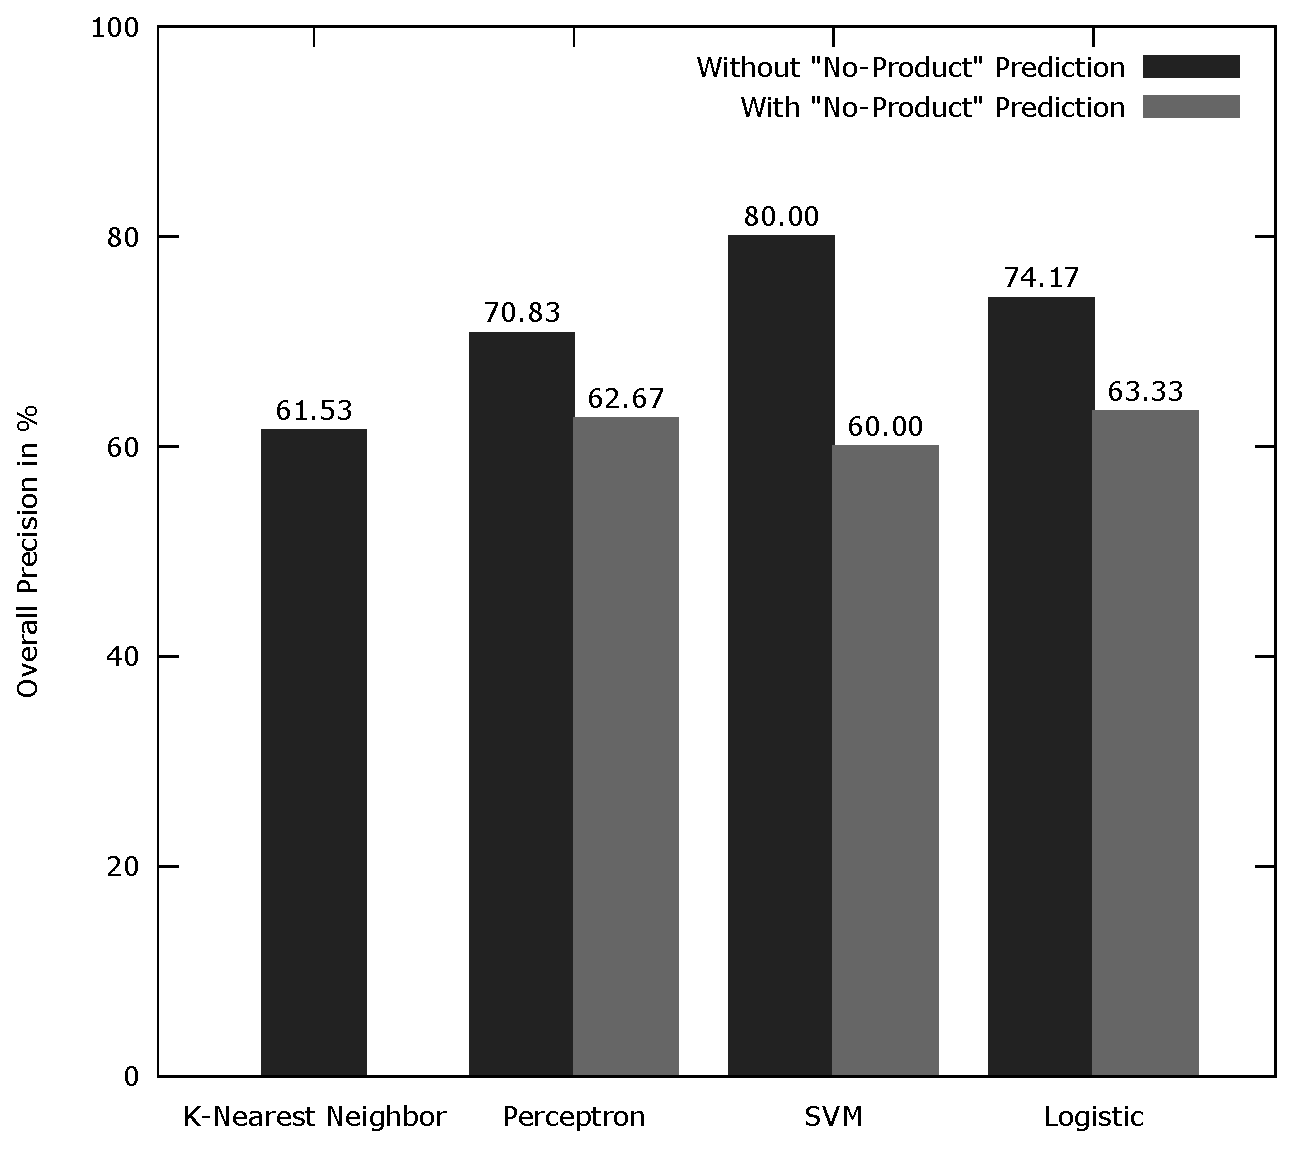
\includegraphics[width=0.5\textwidth]{figures/product_eval.eps}
	\end{center}
	\caption{Comparison of different classifiers and different classification modes}
	\label{fig:product_eval}
\end{figure}

In the following, we take a closer look at some of the design decisions and evaluate their impact on the overall performance.

\subsubsection{Design Decision 1: Feature Selection}
As already mentioned in the Section~\ref{sub:feature-selection}, we use tf-idf feature selection for the product classifier.
Figure~\ref{fig:product_feature_selection} shows the performance of the system for different numbers of features we select.
The best performance was reached when picking only the ten words with the highest tf-idf values, which captures the intuition, that we have to be strict to cope with the \emph{document mismatch problem}.
\begin{figure}[h!]
	\centering
	\begin{subfigure}[t]{0.5\textwidth}
		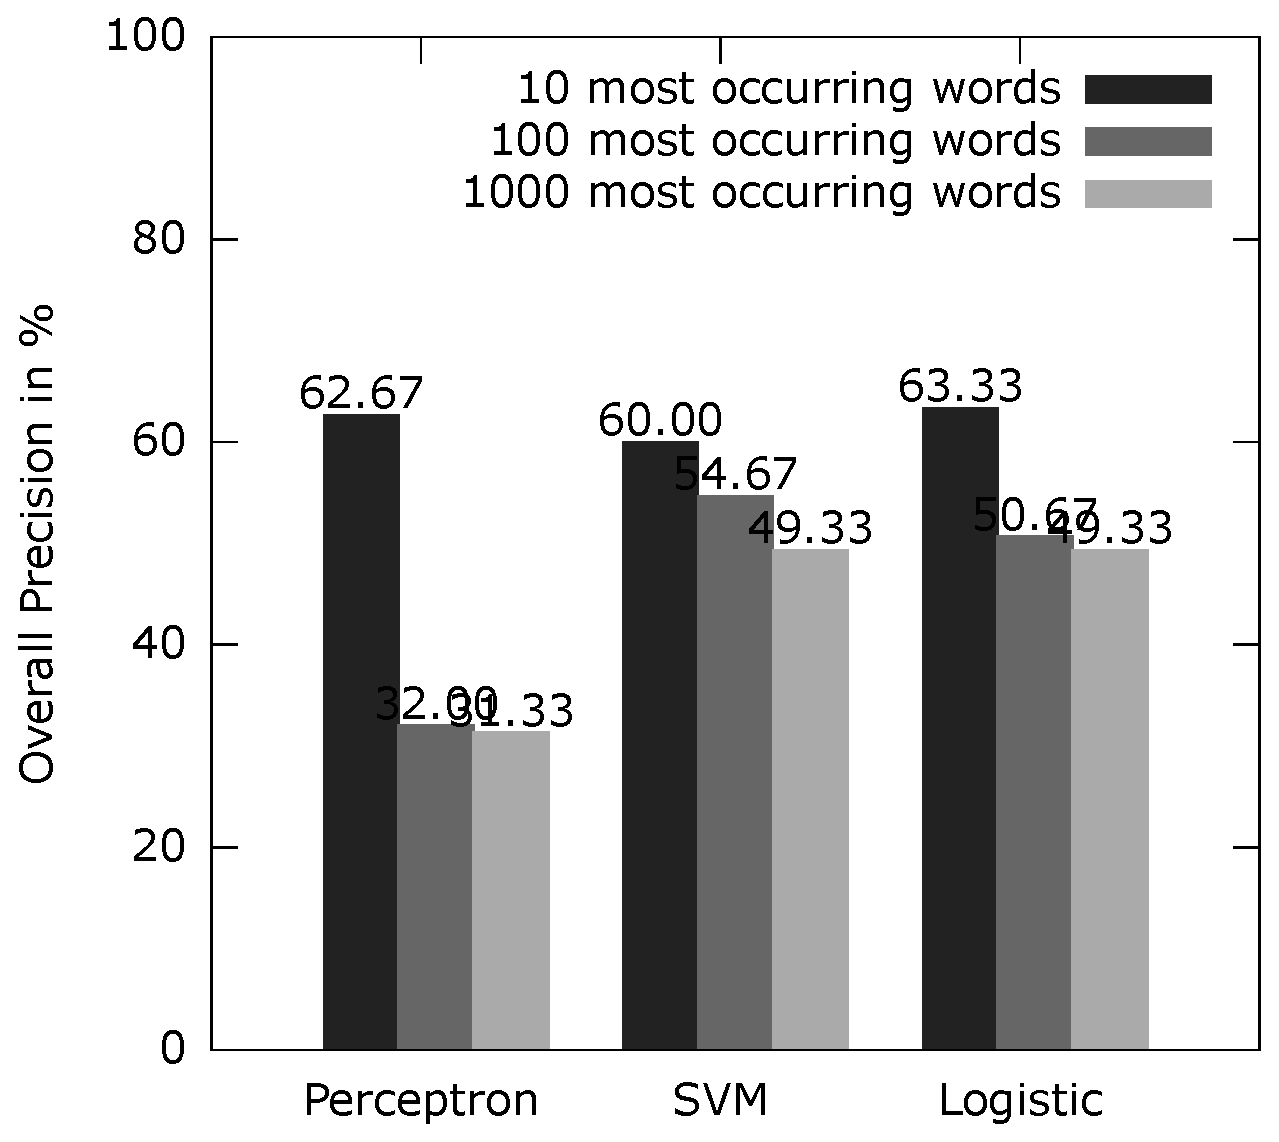
\includegraphics[width=\textwidth]{figures/product_feature_selection_with_none.eps}
		\caption{with ``NONE'' prediction}
	\end{subfigure}~
	\begin{subfigure}[t]{0.5\textwidth}
		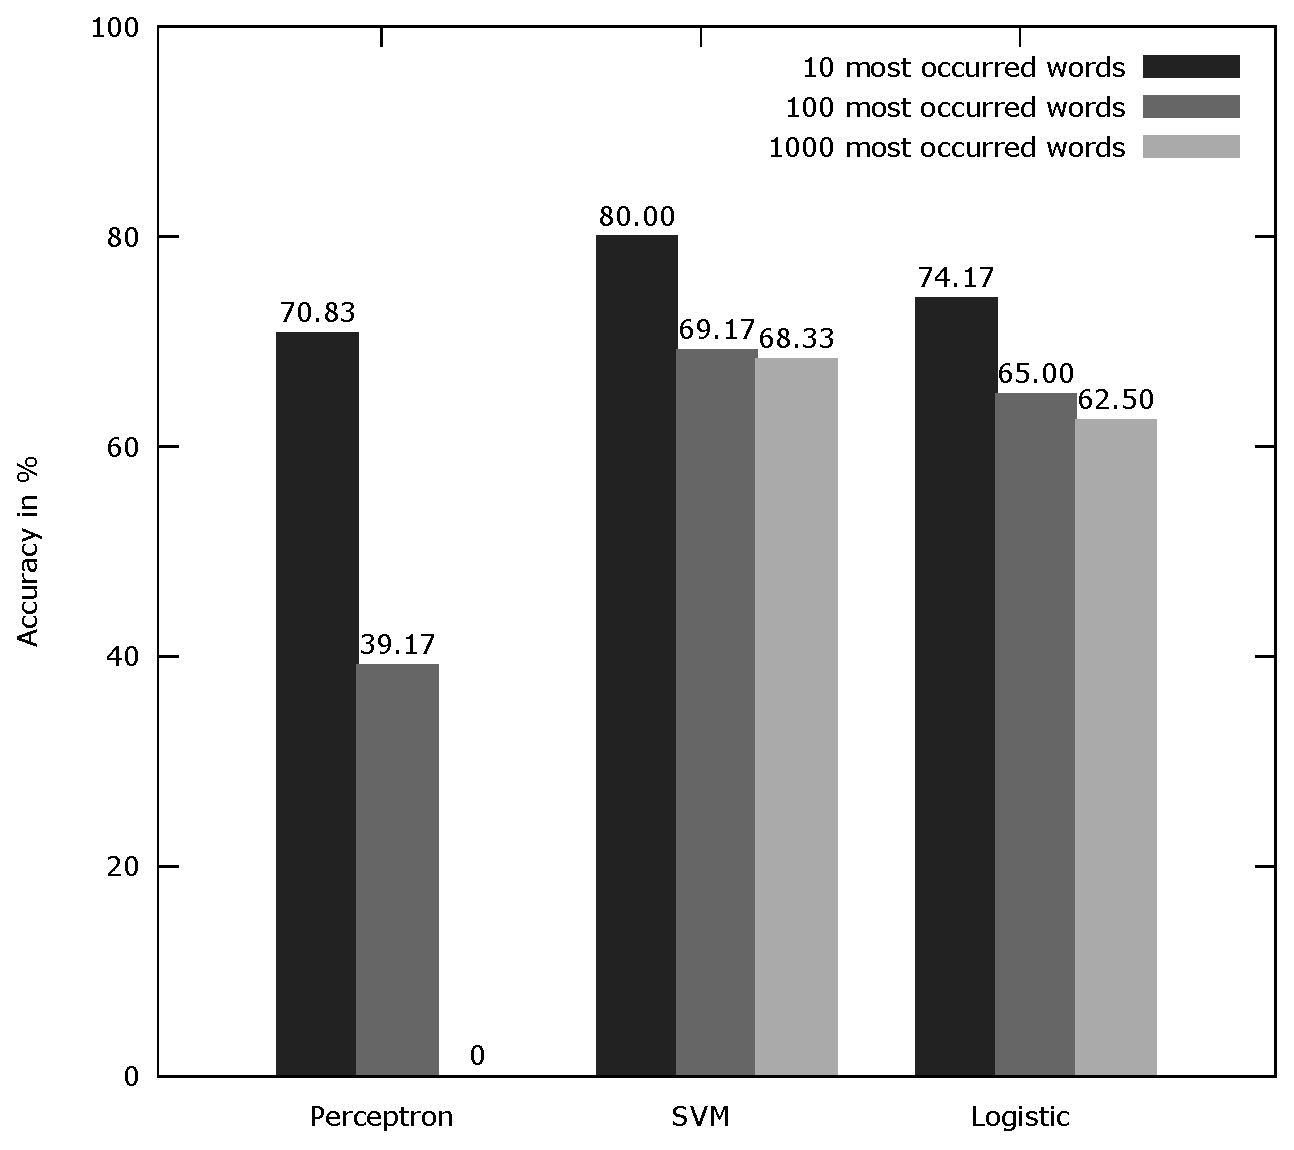
\includegraphics[width=\textwidth]{figures/product_feature_selection_without_none.eps}
		\caption{without ``NONE'' prediction}
	\end{subfigure}
	\caption{Comparison of 10-, 100- and 1,000-most occurring words (with respect to their tf-idf values) selected as features.}
	\label{fig:product_feature_selection}
\end{figure}

\subsubsection{Design Decision 2: Translations and Book Descriptions}
Section~\ref{sub:initial_data_set} described our approach for adapting and increasing the training set.
Compared to a na\"ive approach -- using the brochures as they are -- adding translations and Amazon product descriptions to the training data yields an improvement of 17-20~\% (without ``NONE'' predictions) and 16-28~\% (with ``NONE'' predictions) for the product classifier (see Figure~\ref{fig:product_translate_amazon}).
We believe that this design decision improves the performance for every application of our $NTO$ approach.

\begin{figure}[h!]
	\centering
	\begin{subfigure}[t]{0.5\textwidth}
		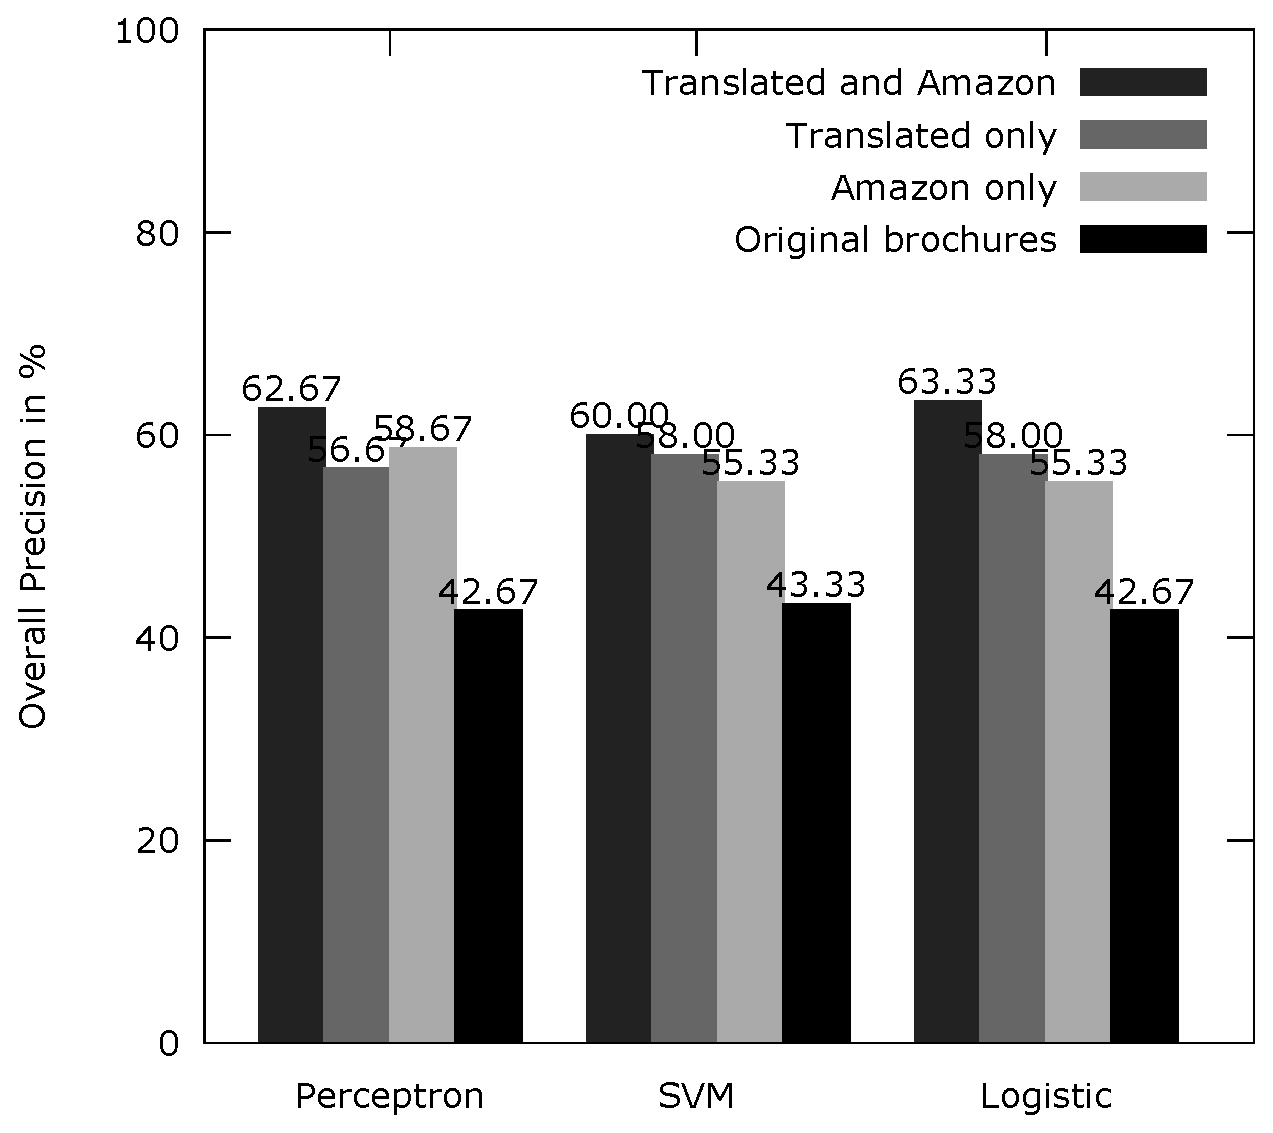
\includegraphics[width=\textwidth]{figures/product_translate_amazon_with_none.eps}
		\caption{with ``NONE'' prediction}
	\end{subfigure}~
	\begin{subfigure}[t]{0.5\textwidth}
		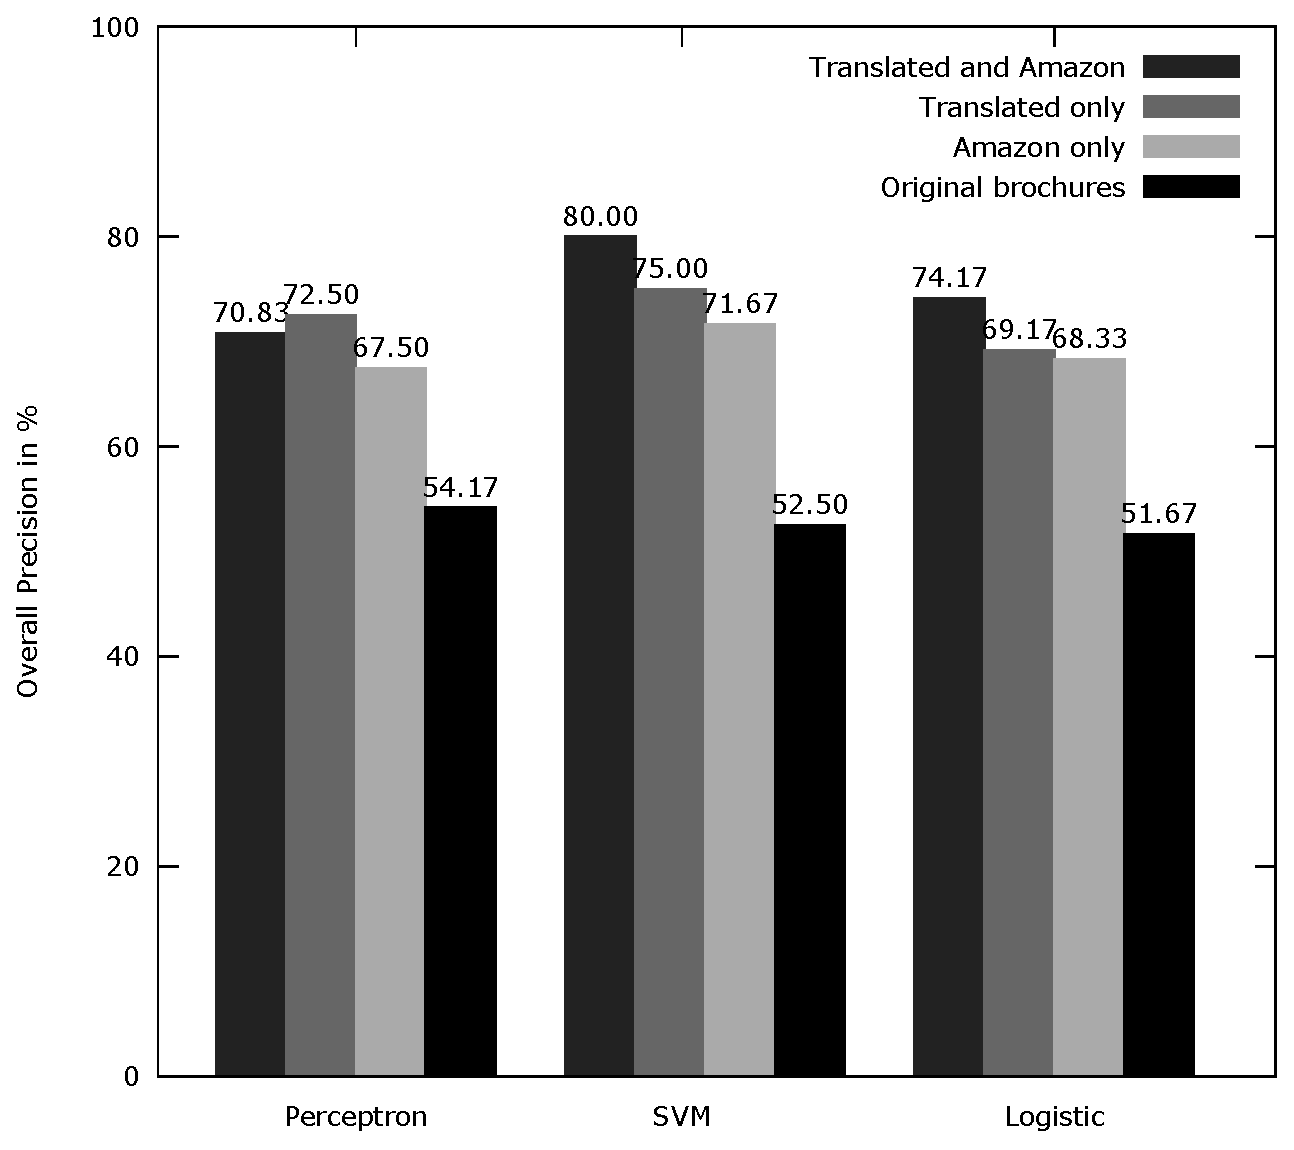
\includegraphics[width=\textwidth]{figures/product_translate_amazon_without_none.eps}
		\caption{without ``NONE'' prediction}
	\end{subfigure}
	\caption{This figure shows different ways to increase the training set size with translations and Amazon book descriptions. Adding both translations and Amazon's texts brings the best performance improvement.}
	\label{fig:product_translate_amazon}
\end{figure}

\subsubsection{Design Decision 3: Two-stage Classifier}
\label{sub:two_stage_classifier}

A central point of our work was to propose a two-stage classifier for the \nto problem.
To evaluate this approach we compare our two-stage classifier against a single classifier.
The single classifier was trained using both the brochures and the tagged LinkedIn posts as the training data and directly returns a product.
By using both the brochures and the tagged posts we make sure, that both classifiers learn on the same amount of data.
% This one-stage classifier is identical to our product classifier.

For that evaluation we change the test set annotations in the way, that if an annotated post was been classified as ``no-demand'', the product classification is ignored, and ``NONE'' is used instead.
In this way we can compare the predictions of the product classifier (which is either ``NONE'' or one of the products) with the predictions of the two-stage classifier (which is also either ``NONE'' or one of the products).
Because both classifiers are trained on the LinkedIn posts, we do a ten-fold cross validation on the LinkedIn posts.
As shown in Table~\ref{table:two_stage_eval} the two-stage classifier yields an improvement of about 12~\%.

These values confirm our concept that demand and product classification are two different things, and should be learned separately to increase the performance of the system.

\begin{table}
	\centering
	\begin{tabular}{c|c}
		\hline
		Product classification & Two-stage classification \\
		\hline \hline
		69.73\% & 81.35\% \\
		\hline
	\end{tabular}
	\caption{Comparison of the standalone product classification with the two-stage classification.}
	\label{table:two_stage_eval}
\end{table}
